\documentclass[a4paper, 12pt]{article}
\usepackage[UTF8]{ctex}
\title{实验报告}
\author{23020007067 李子昊}
\date{\today}
\usepackage{color}    
\usepackage{float}
\usepackage{graphicx}
\usepackage[left=2cm,right=2cm,top=2cm,bottom=2cm,head=1cm,headsep=0.5cm,foot=1cm]{geometry}
\usepackage{hyperref}
\usepackage{indentfirst}
\usepackage{booktabs}
\hypersetup{hidelinks,
	colorlinks=true,
	allcolors=black,
	pdfstartview=Fit,
	breaklinks=true}
    
\begin{document}
\maketitle

\pagenumbering{roman}
\large \tableofcontents
\newpage
\pagenumbering{arabic}
 
 \section{课后练习}
\subsection{调试及性能分析练习}
\noindent 1.使用python中自带的pdb--help进行调试。
\begin{figure}[H]
  \centering
  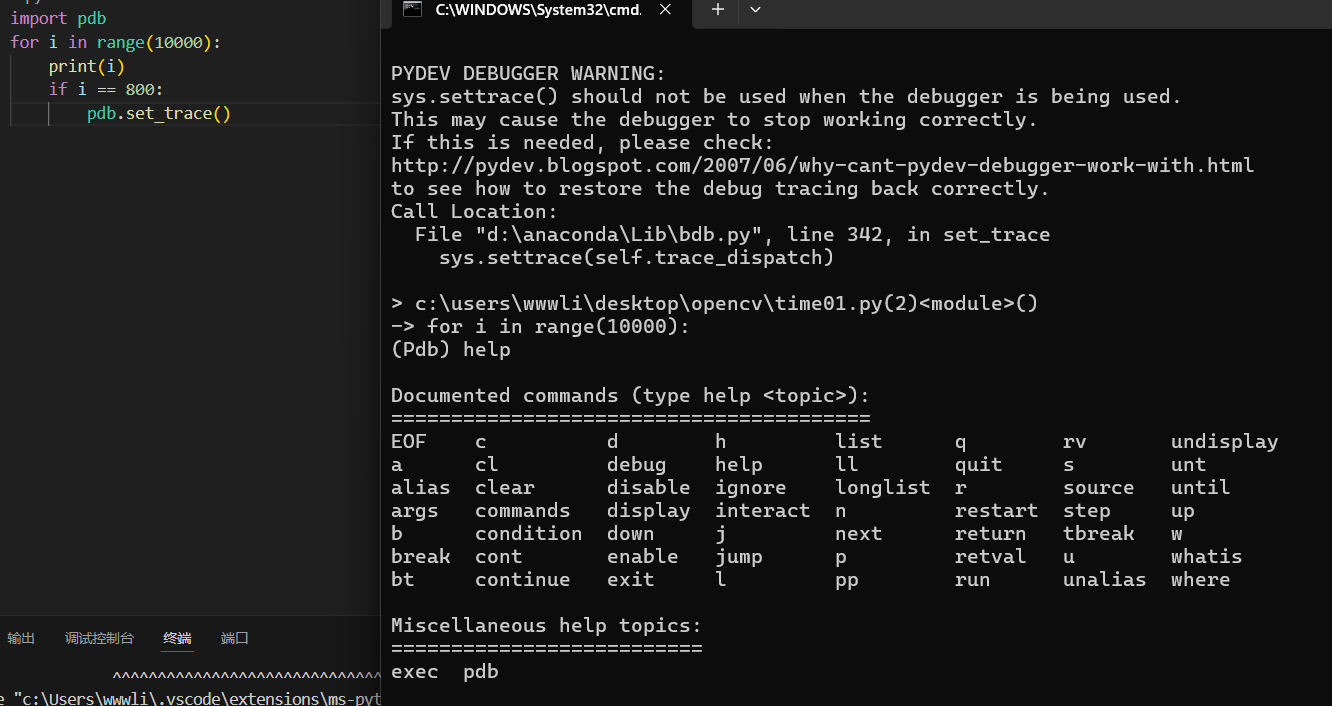
\includegraphics[width=\textwidth]{屏幕截图 2024-09-15 153834.png}
  \caption{题目一}
\end{figure}

2.使用 Linux 上的 journalctl 或 macOS 上的 log show 命令来获取最近一天中超级用户的登录信息及其所执行的指令。如果找不到相关信息,您可以执行一些无害的命令,例如 sudo ls 然后再次查看。
\begin{figure}[H]
  \centering
  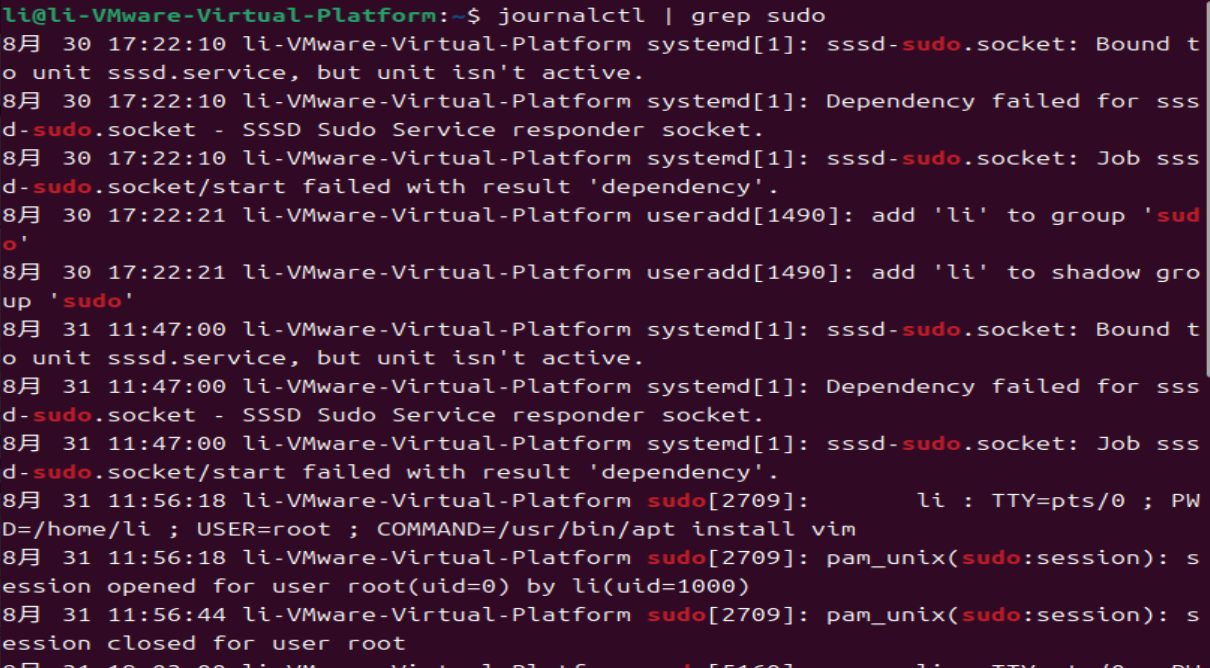
\includegraphics[width=\textwidth]{屏幕截图 2024-09-15 115738.png}
  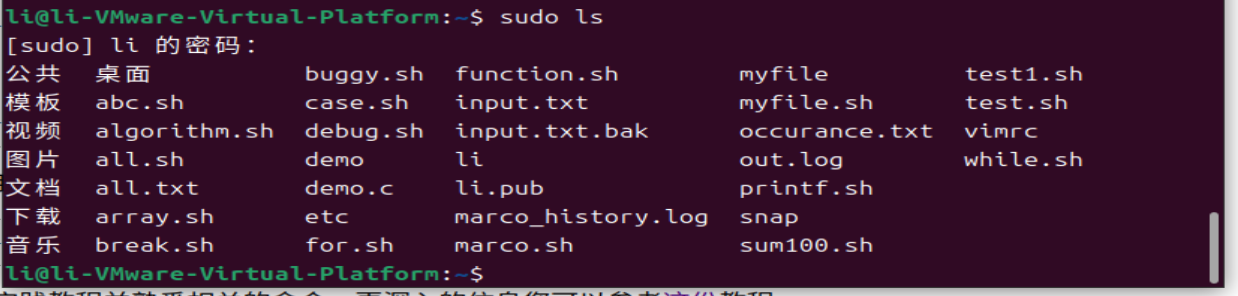
\includegraphics[width=\textwidth]{屏幕截图 2024-09-15 115836.png}
  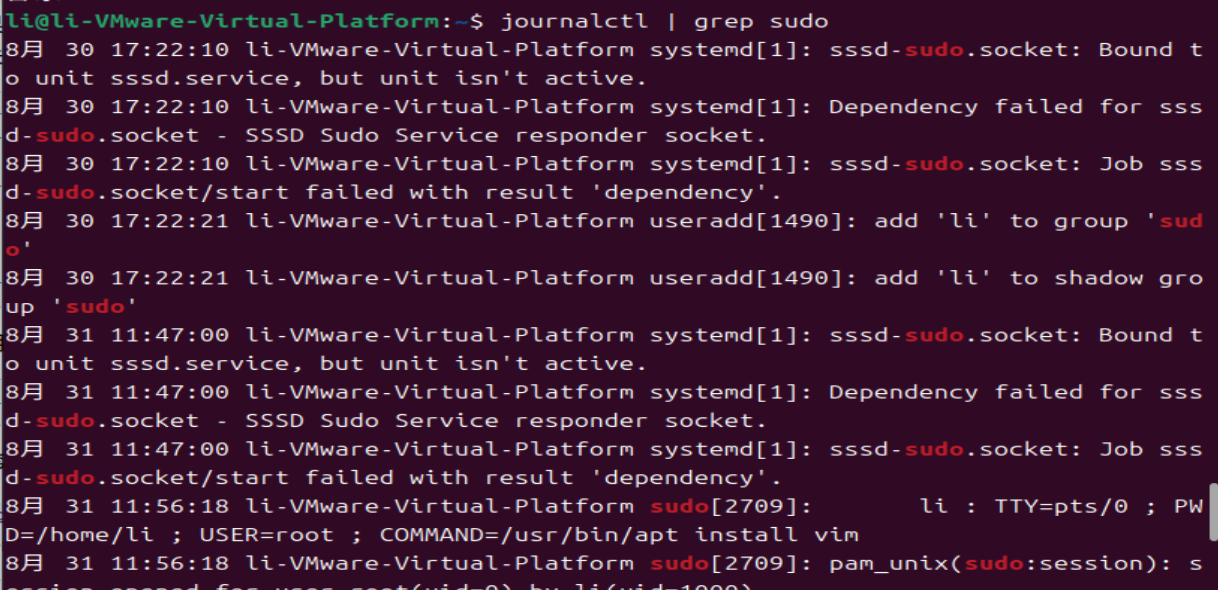
\includegraphics[width=\textwidth]{屏幕截图 2024-09-15 115913.png}
  \caption{题目二}
\end{figure}

3.请阅读 可逆调试 并尝试创建一个可以工作的例子(使用 rr 或 RevPDB)。
\begin{figure}[H]
  \centering
  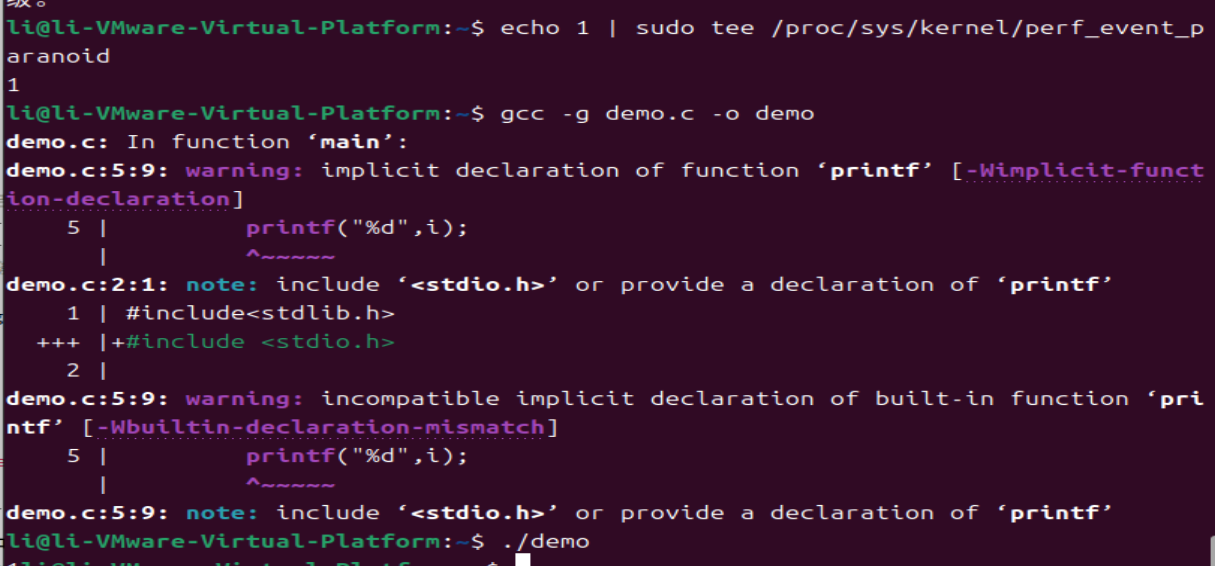
\includegraphics[width=\textwidth]{屏幕截图 2024-09-15 120117.png}
  \caption{题目三}
\end{figure}

4.使用python语句判断程序运行了多长时间。

\begin{figure}[H]
  \centering
  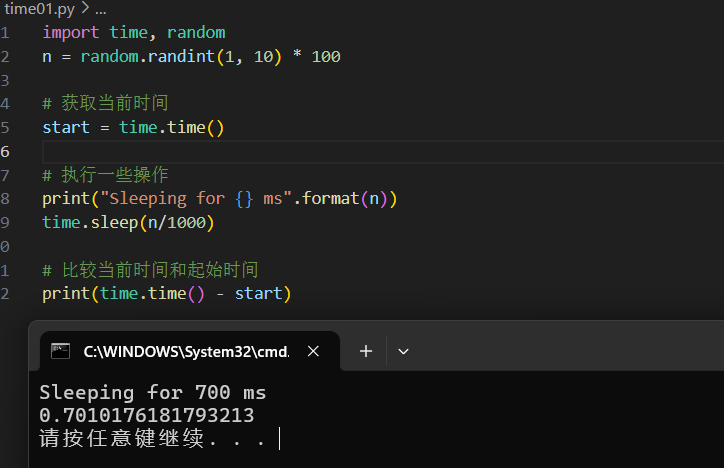
\includegraphics[width=\textwidth]{屏幕截图 2024-09-15 141747.png}
  \caption{题目四}
\end{figure}

\subsection{元编程练习}
1.大多数的 makefiles 都提供了 一个名为 clean 的构建目标,这并不是说我们会生成一个名为 clean 的文件,而是我们可以使用它清理文件,让 make 重新构建。您可以理解为它的作用是“撤销”所有构建步骤。在上面的 makefile 中为 paper.pdf 实现一个 clean 目标。您需要将构建目标设置为 phony。您也许会发现 git ls-files 子命令很有用。其他一些有用的 make 构建目标可以在这里找到。
\begin{figure}[H]
  \centering
  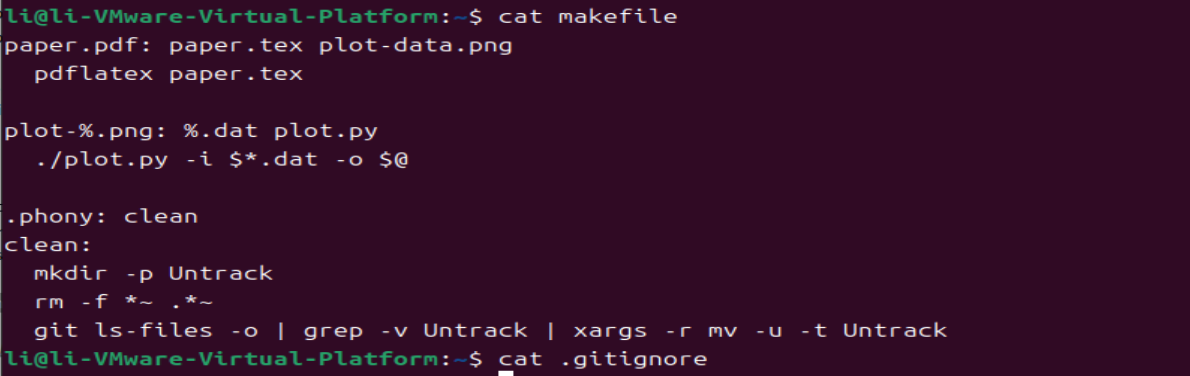
\includegraphics[width=\textwidth]{屏幕截图 2024-09-15 215813.png}
  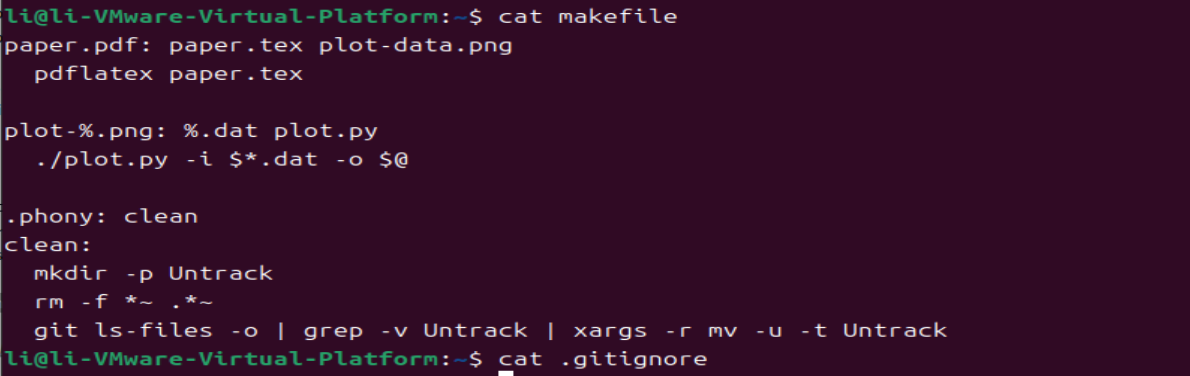
\includegraphics[width=\textwidth]{屏幕截图 2024-09-15 215813.png}
  \caption{make}
\end{figure}



\subsection{PyTorch 编程练习}
1.求出tensor的一阶导、二阶导和三阶导
\begin{figure}[H]
  \centering
  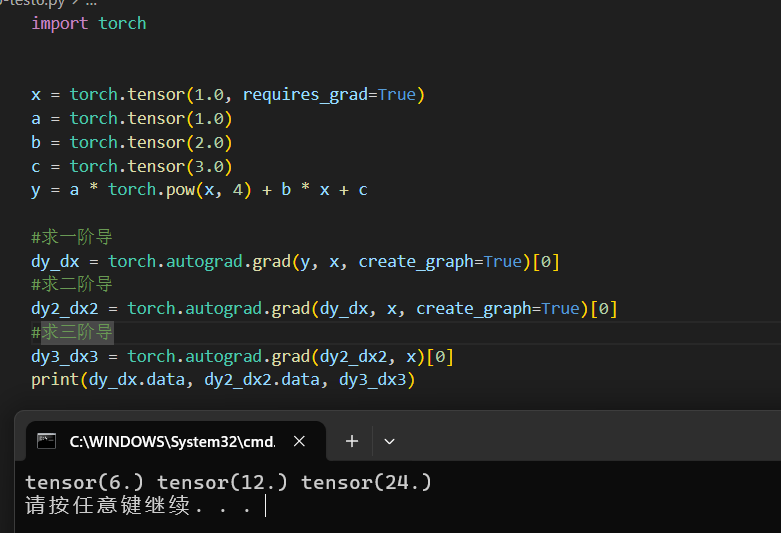
\includegraphics[width=\textwidth]{屏幕截图 2024-09-15 110908.png}
  \caption{torch.autograd.grad}
\end{figure}

2.实现张量的拼接+升维
\begin{figure}[H]
  \centering
  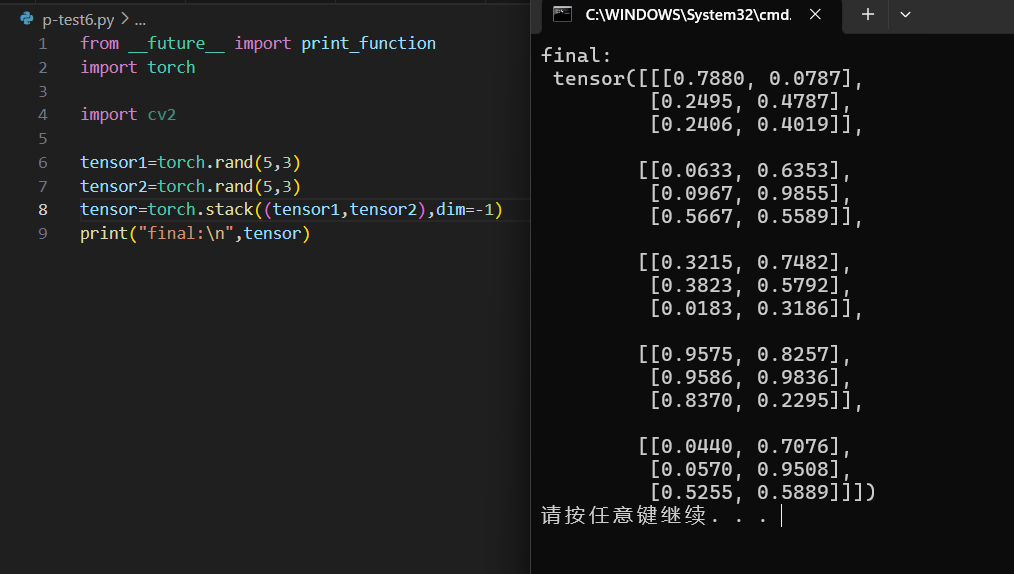
\includegraphics[width=\textwidth]{屏幕截图 2024-09-15 110619.png}
  \caption{torch.stack}
\end{figure}

3.实现张量的行列交换
\begin{figure}[H]
  \centering
  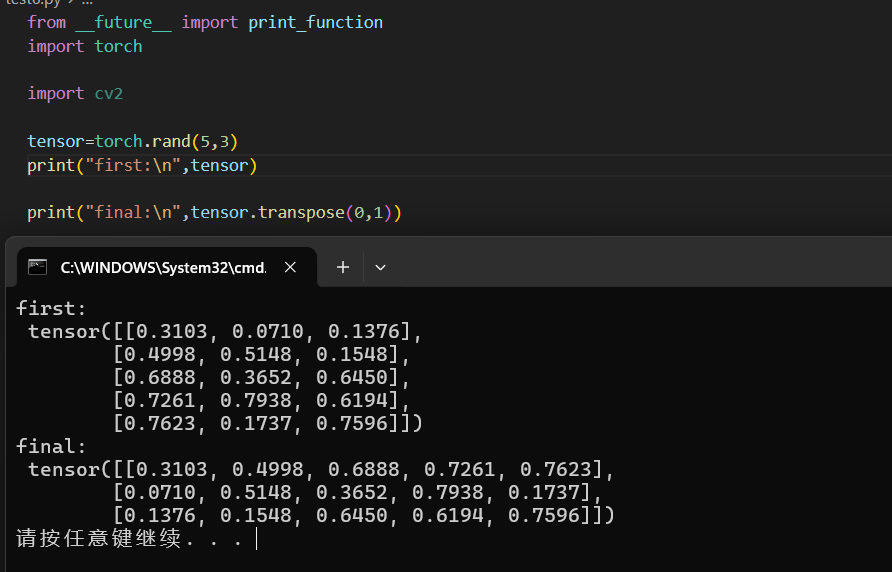
\includegraphics[width=\textwidth]{屏幕截图 2024-09-15 110337.png}
  \caption{A.transpose(0,1)}
\end{figure}

\section{实例展示}
 \subsection{调试及性能分析实例展示}
\begin{table}[H]
\centering
\caption{ {\color{red}PyTorch实例展示}}
\begin{tabular}{ccc}
\toprule
1& journalctl | grep sudo &获取登录信息及指令  \\
\hline
2&sudo ls & 查看文件   \\ \hline
3&sudo tee /proc/sys/kernel/perf\_event\_paranoid &  向文件输出内容   \\ \hline
4&gcc -g demo.c -o demo& 编译运行demo.c    \\ \hline
 5 & pdb.set\_trace() &   启动 pdb 调试 \\ \hline
6& pdb中ll  &   查看上下文  \\ \hline
7& pdb中help & 查看帮助   \\  \hline
8& pdb中 c  & 继续执行程序  \\  \hline
9&cProfile.run()  &  查看代码总的效率以及各个部分的效率  \\ \hline
10&stress -c 3 &   创建负载
  \\
\bottomrule
\end{tabular}
\end{table}

1.journalctl | grep sudo :获取登录信息及指令
\begin{figure}[H]
  \centering
  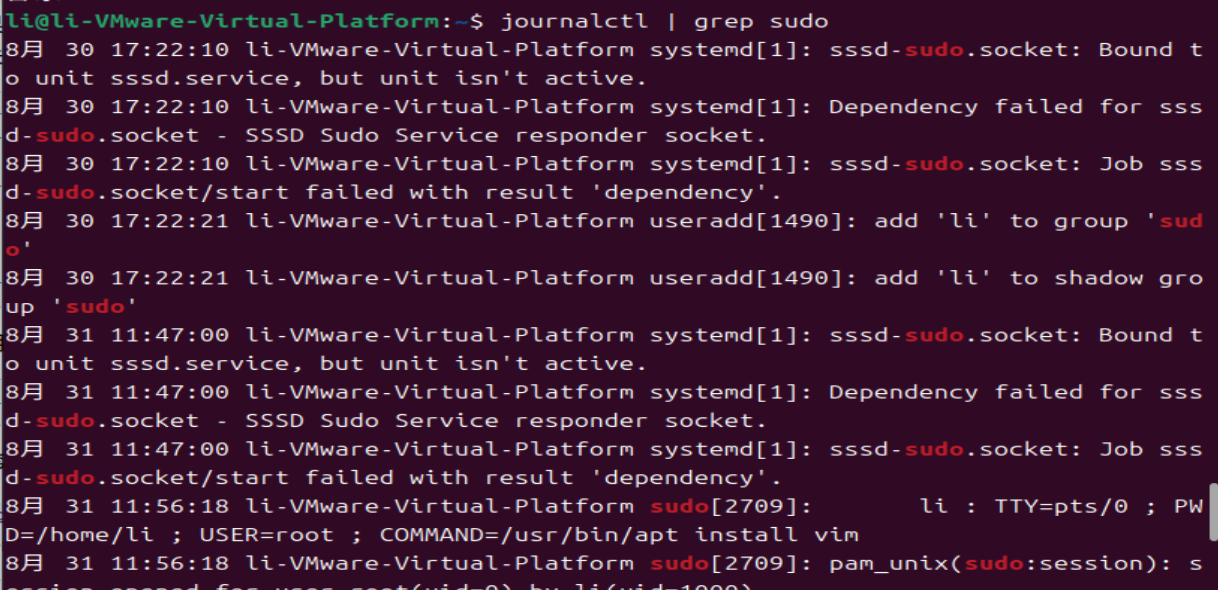
\includegraphics[width=\textwidth]{屏幕截图 2024-09-15 115913.png}
  \caption{journalctl | grep sudo}
\end{figure}


2.sudo ls : 查看文件
\begin{figure}[H]
  \centering
  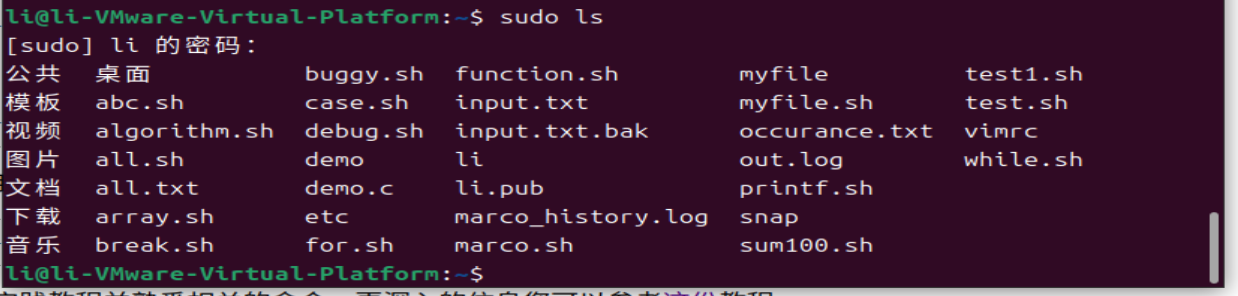
\includegraphics[width=\textwidth]{屏幕截图 2024-09-15 115836.png}
  \caption{sudo ls}
\end{figure}

3.sudo tee /proc/sys/kernel/perf\_event\_paranoid
\begin{figure}[H]
  \centering
  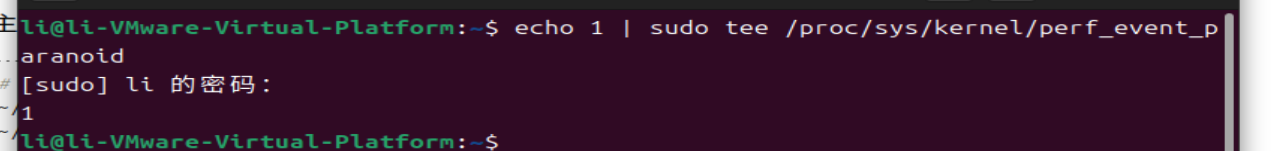
\includegraphics[width=\textwidth]{屏幕截图 2024-09-15 162052.png}
  \caption{sudo tee /proc/sys/kernel/perf\_event\_paranoid}
\end{figure}

4.gcc -g demo.c -o demo:编译运行demo.c 
\begin{figure}[H]
  \centering
  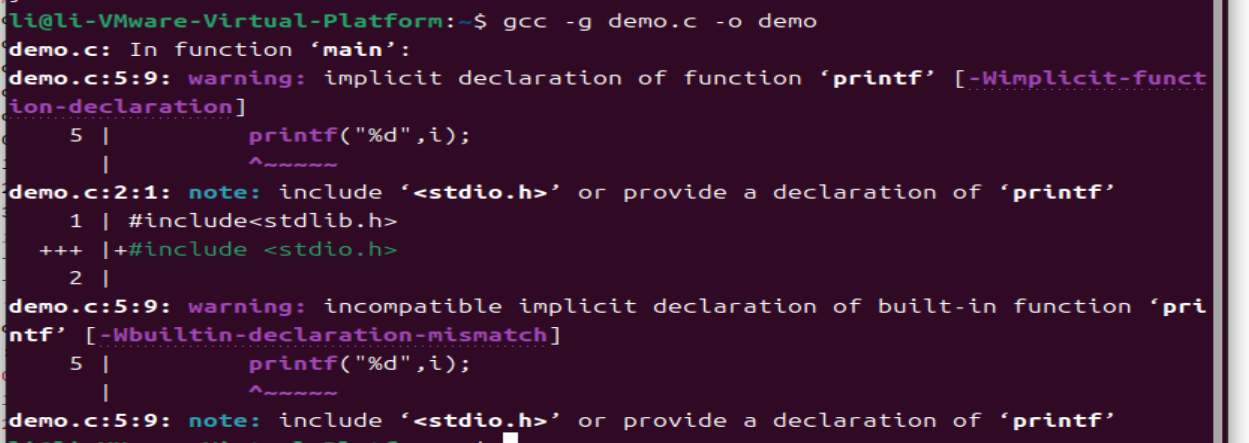
\includegraphics[width=\textwidth]{屏幕截图 2024-09-15 162147.png}
  \caption{gcc -g demo.c -o demo}
\end{figure}

5.pdb.set\_trace():启动 pdb 调试
\begin{figure}[H]
  \centering
  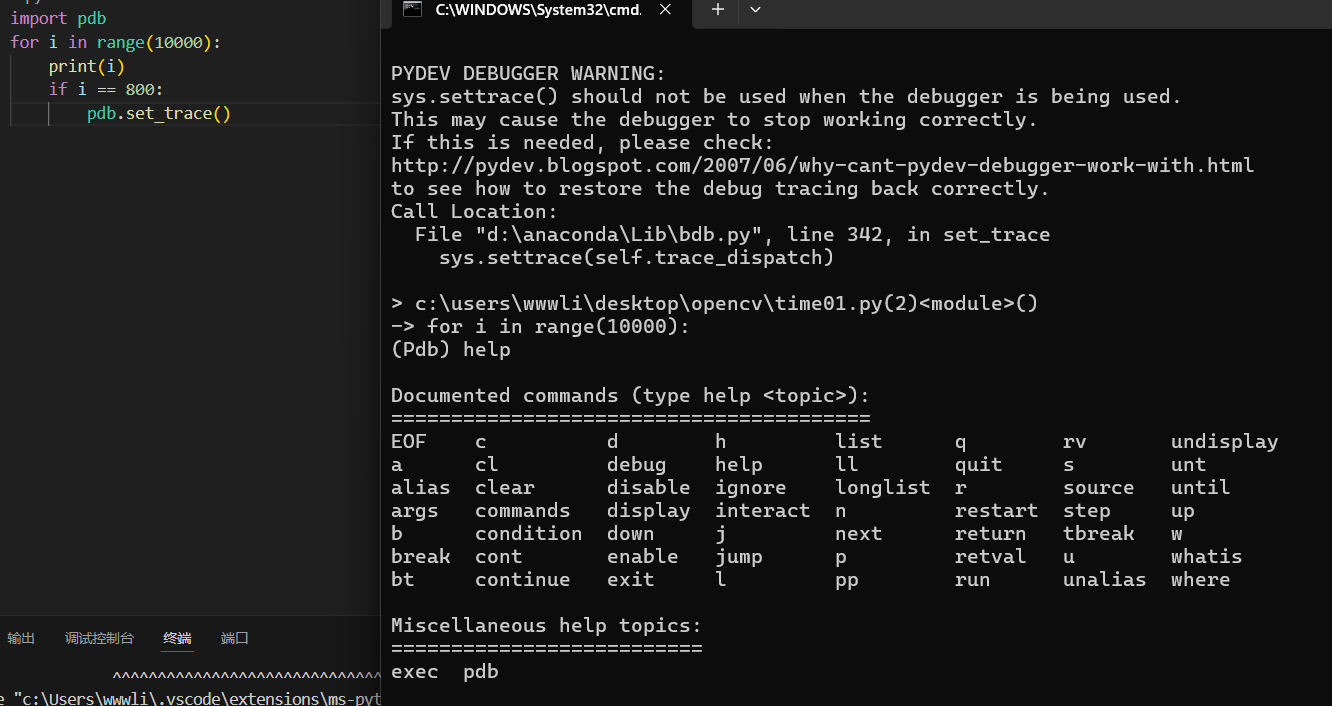
\includegraphics[width=\textwidth]{屏幕截图 2024-09-15 153834.png}
  \caption{pdb.set\_trace()}
\end{figure}

6.pdb中ll:查看上下文
\begin{figure}[H]
  \centering
  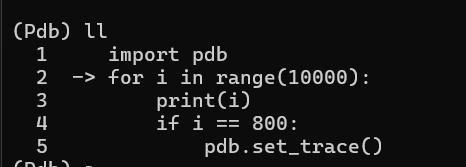
\includegraphics[width=\textwidth]{屏幕截图 2024-09-15 155054.png}
  \caption{ll}
\end{figure}

7.pdb中help:查看帮助   
\begin{figure}[H]
  \centering
  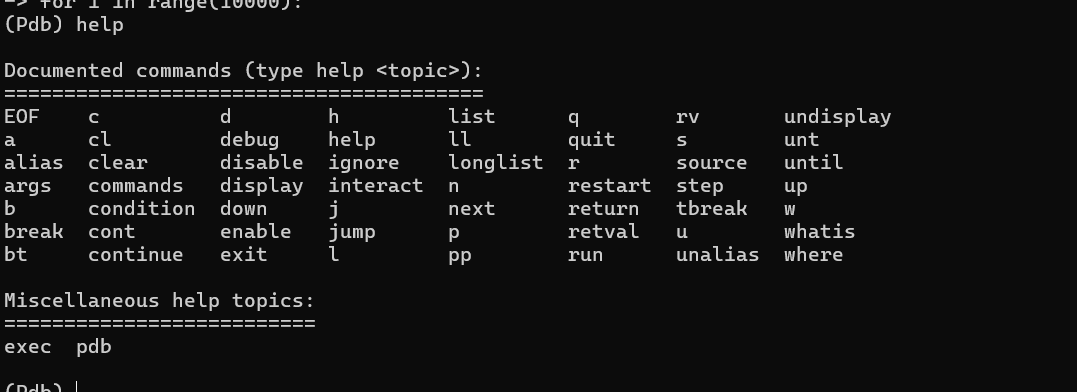
\includegraphics[width=\textwidth]{屏幕截图 2024-09-15 162427.png}
  \caption{help}
\end{figure}
8.pdb中 c:继续执行程序  
\begin{figure}[H]
  \centering
  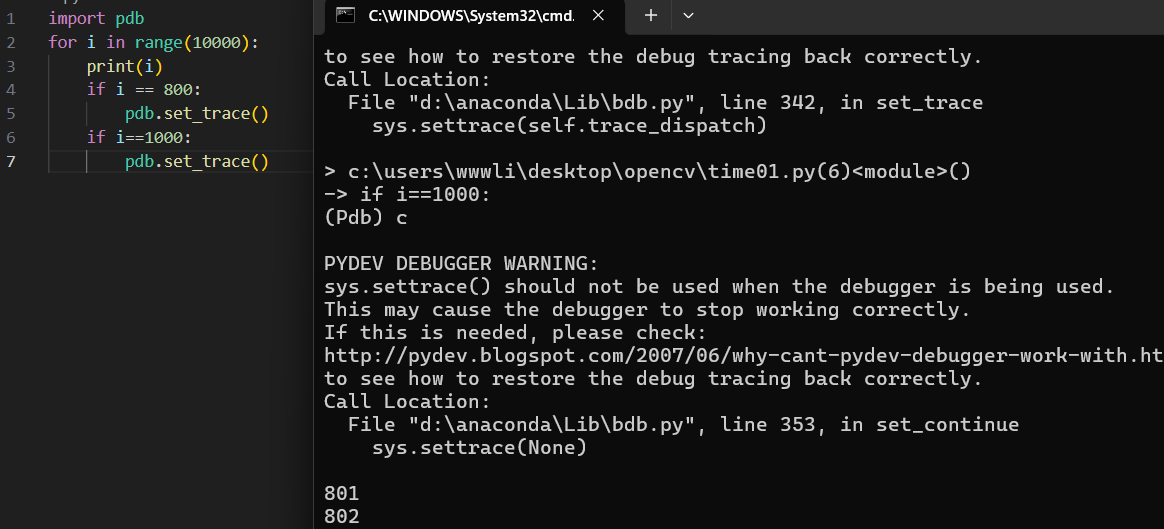
\includegraphics[width=\textwidth]{屏幕截图 2024-09-15 162600.png}
  \caption{c}
\end{figure}

9.cProfile.run():查看代码总的效率以及各个部分的效率 
\begin{figure}[H]
  \centering
  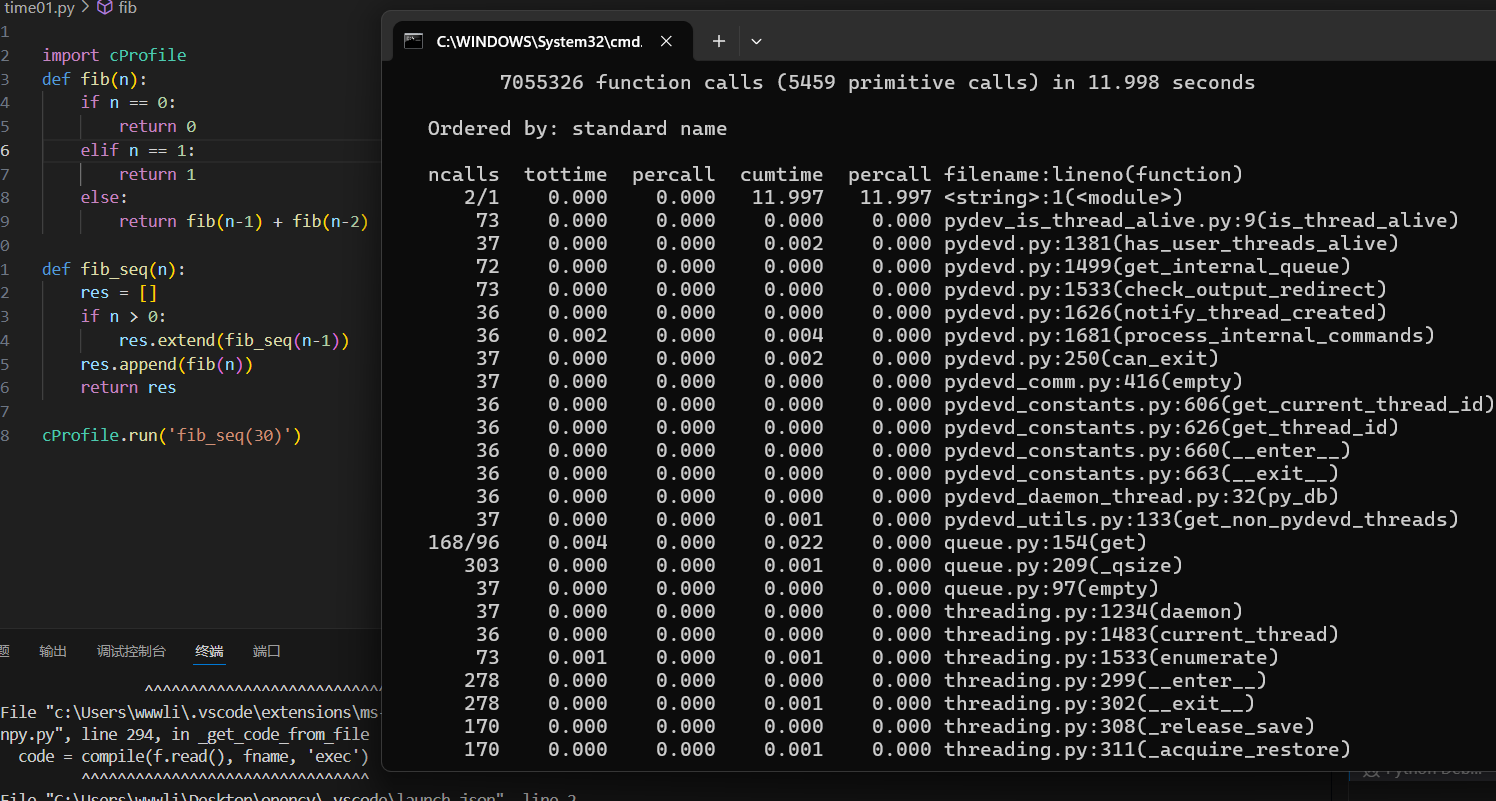
\includegraphics[width=\textwidth]{屏幕截图 2024-09-15 153604.png}
  \caption{cProfile.run()}
\end{figure}

10.stress -c 3:创建负载
\begin{figure}[H]
  \centering
  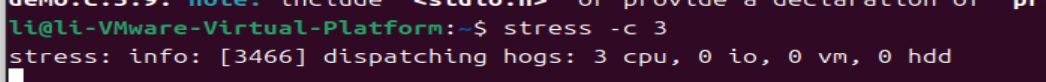
\includegraphics[width=\textwidth]{屏幕截图 2024-09-15 162844.png}
  \caption{stress -c 3}
\end{figure}

\subsection{元编程实例展示}

\begin{table}[H]
\centering
\caption{ {\color{red}PyTorch实例展示}}
\begin{tabular}{ccc}
\toprule
1&\_\_init\_\_和\_\_call\_\_ &类的初始化   \\
\hline
2&def \_\_get\_\_(self, instance, cls) & 装饰器   \\ \hline
3&template<typename T, std::size_t N> & 混合元编程   \\ \hline
4&constexpr T Factorial(T x) & 类元编程    \\ \hline
 5 & struct remove_reference<_Ty&&>  &   类型元编程  \\ \hline
6& func=decorator(func) &   装饰器表示  \\ 
\bottomrule
\end{tabular}
\end{table}


1.一个类只能有一个实例
\begin{figure}[H]
  \centering
  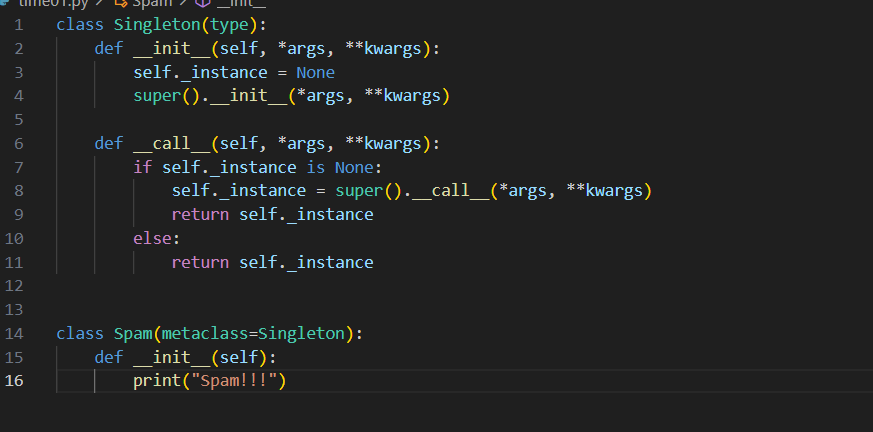
\includegraphics[width=\textwidth]{屏幕截图 2024-09-15 183935.png}
  \caption{ \_\_init\_\_和\_\_call\_\_}
\end{figure}

2.c++值元编程
\begin{figure}[H]
  \centering
  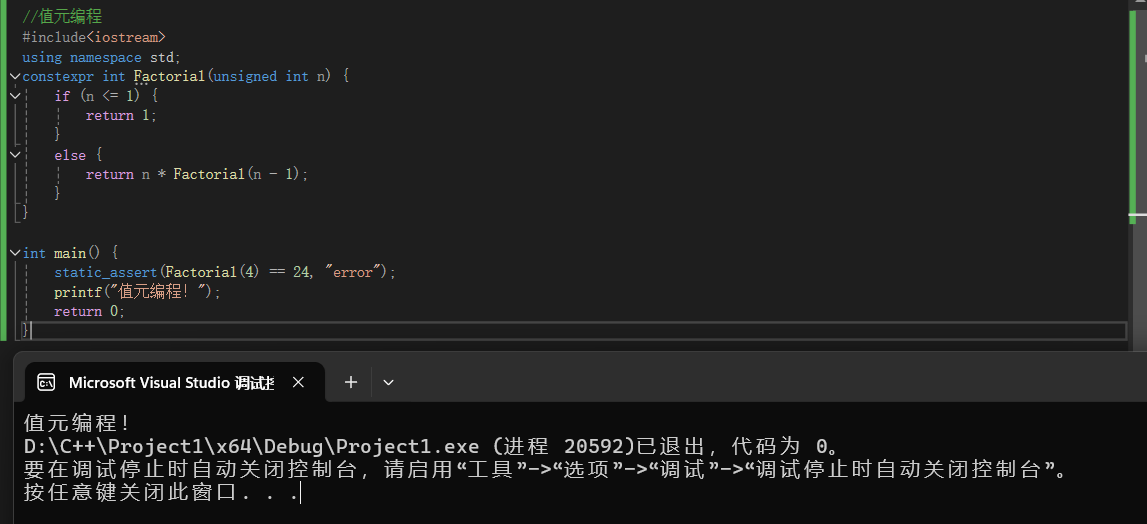
\includegraphics[width=\textwidth]{屏幕截图 2024-09-15 184403.png}
  \caption{ c++值元编程}
\end{figure}


3.c++混合元编程
\begin{figure}[H]
  \centering
  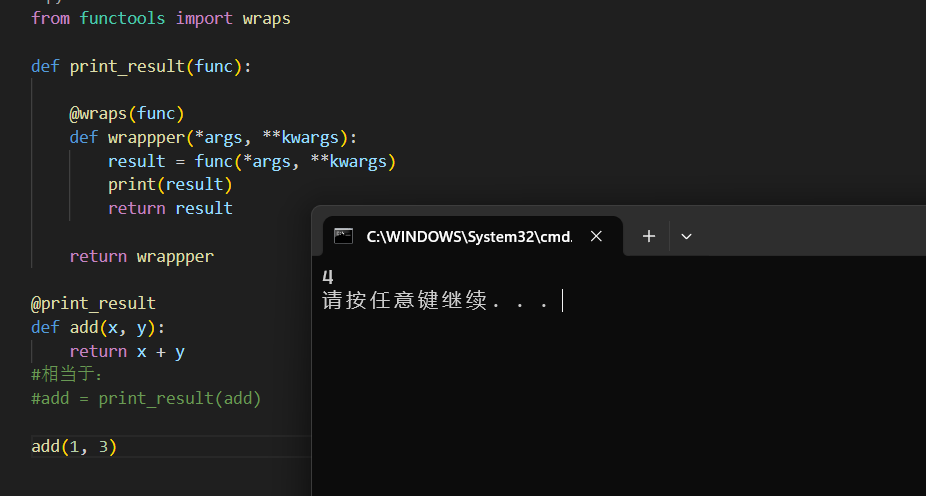
\includegraphics[width=\textwidth]{屏幕截图 2024-09-15 185638.png}
  \caption{ c++混合元编程}
\end{figure}


4.装饰器
\begin{figure}[H]
  \centering
  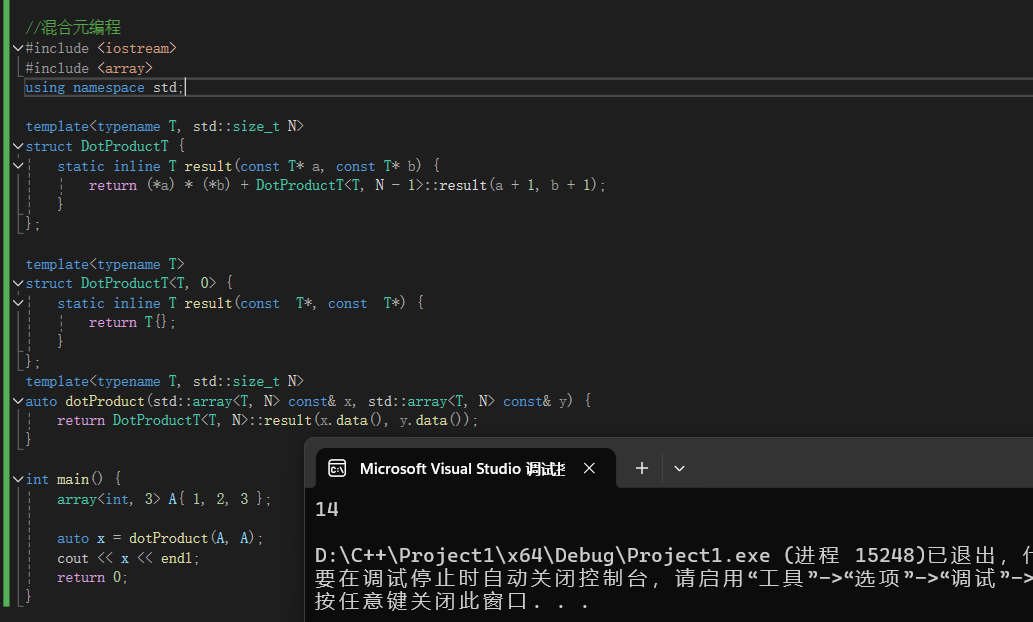
\includegraphics[width=\textwidth]{屏幕截图 2024-09-15 184654.png}
  \caption{ 装饰器}
\end{figure}

5.func=decorator(func)
\begin{figure}[H]
  \centering
  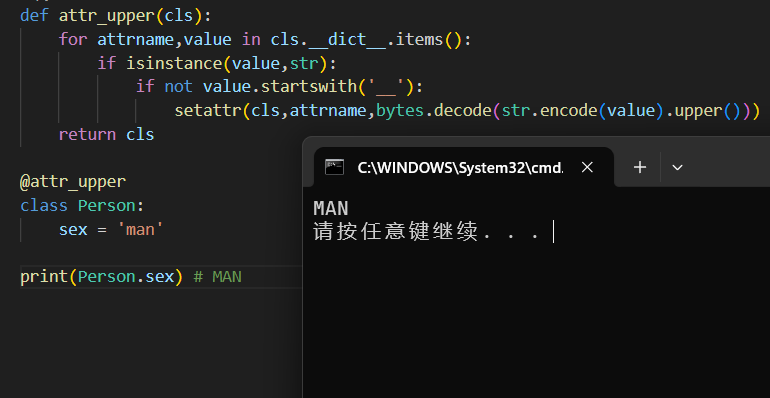
\includegraphics[width=\textwidth]{屏幕截图 2024-09-15 185701.png}
  \caption{ func=decorato(func)}
\end{figure}

\subsection{PyTorch 编程实例展示}
\begin{table}[H]
\centering
\caption{ {\color{red}PyTorch实例展示}}
\begin{tabular}{ccc}
\toprule
1&torch.empty() &声明一个未初始化的矩阵   \\
\hline
2&torch.rand() & 随机初始化一个矩阵    \\ \hline
3&torch.zeros() &  创建数值皆为 0 的矩阵   \\ \hline
4&torch.tensor()& 直接传递 tensor 数值来创建    \\ \hline
 5 & tensor.new\_ones() &   根据已有的 tensor 变量创建新的 tensor 变量  \\ \hline
6& torch.randn\_like(old\_tensor) &   保留相同的尺寸大小  \\ \hline
7& tensor1.add\_(tensor2) & 直接修改 tensor 变量   \\  \hline
8& tensor3.size() &对 tensors 的尺寸大小获取  \\  \hline
9&A.backward(torch.tensor(1.)) &  计算梯度  \\ \hline
10&torch.range(begin,end,step) &   起始位置,终止位置和步长 \\ \hline
11&torch.mv(A,B) &   矩阵与向量相乘  \\ \hline
 12& A.numpy() & 将Tensor转化为Numpy类型  \\ \hline
 13&torch.diag(A) & 取A对角线元素形成一个一维向量 \\ \hline
 14&A.transpose(0,1) & 行列交换  \\ \hline
 15&torch.stack& 拼接+升维 \\ \hline
 16& autograd.grad& 求导   \\
\bottomrule
\end{tabular}
\end{table}

1.torch.empty():声明一个未初始化的矩阵
\begin{figure}[H]
  \centering
  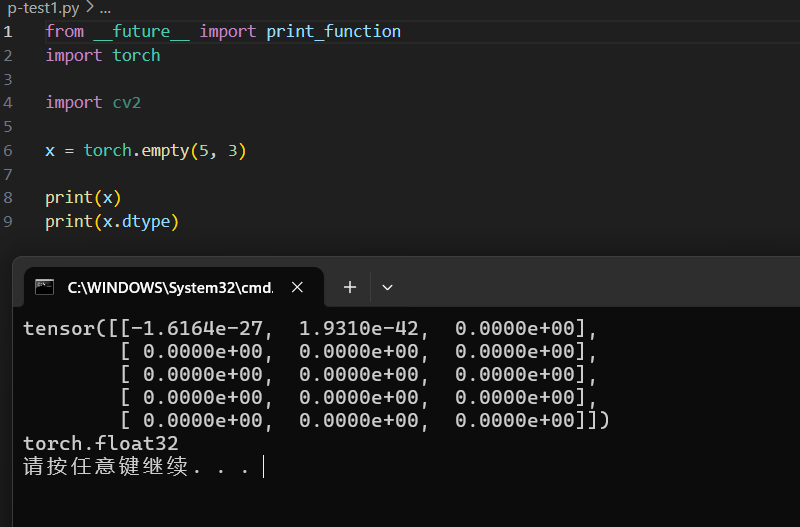
\includegraphics[width=\textwidth]{屏幕截图 2024-09-15 102104.png}
  \caption{torch.empty()}
\end{figure}

2.torch.rand():随机初始化一个矩阵
\begin{figure}[H]
  \centering
  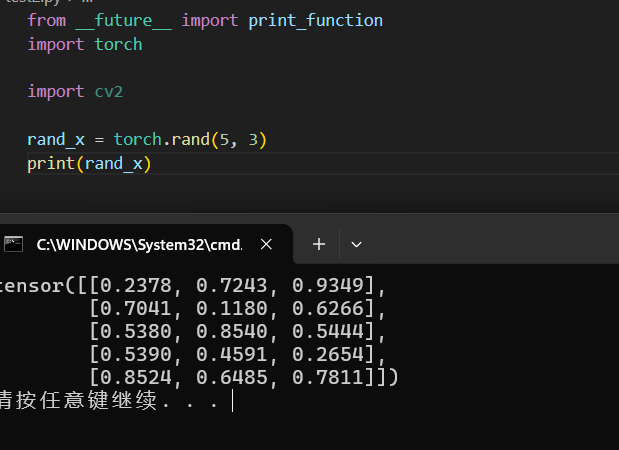
\includegraphics[width=\textwidth]{屏幕截图 2024-09-15 102156.png}
  \caption{torch.rand()}
\end{figure}

3.torch.zeros():创建数值皆为 0 的矩阵
\begin{figure}[H]
  \centering
  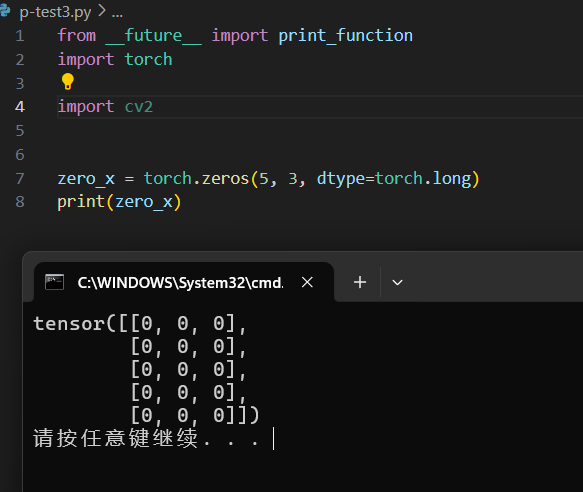
\includegraphics[width=\textwidth]{屏幕截图 2024-09-15 102246.png}
  \caption{torch.zeros()}
\end{figure}

4.torch.tensor():直接传递 tensor 数值来创建
\begin{figure}[H]
  \centering
  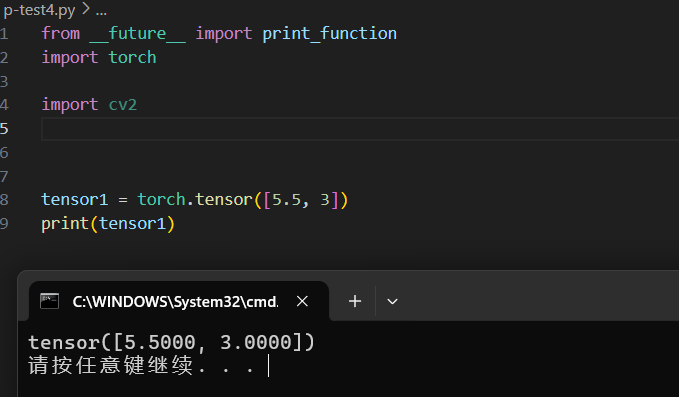
\includegraphics[width=\textwidth]{屏幕截图 2024-09-15 102342.png}
  \caption{torch.tensor()}
\end{figure}

5.tensor.new\_ones():new\_*() 方法需要输入尺寸大小
\begin{figure}[H]
  \centering
  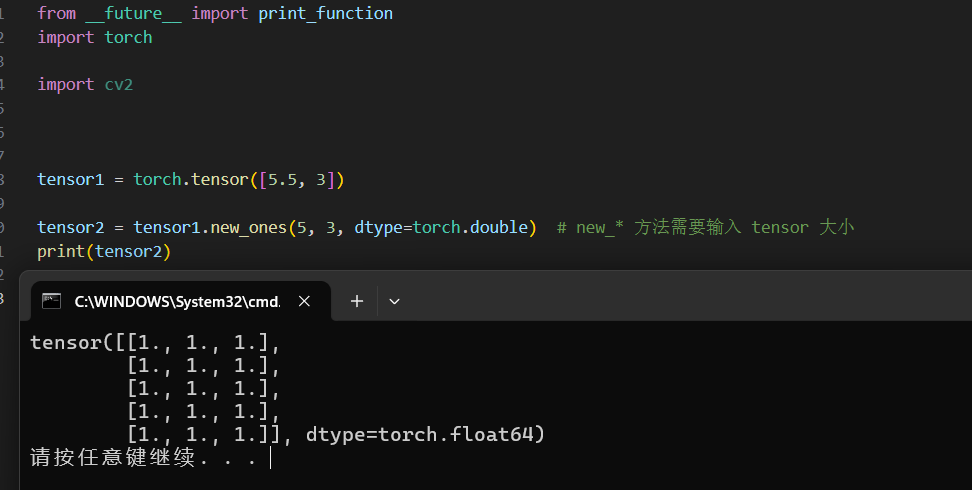
\includegraphics[width=\textwidth]{屏幕截图 2024-09-15 103948.png}
  \caption{torch.new\_ones()}
\end{figure}

6.torch.randn\_like(old\_tensor):保留相同的尺寸大小
\begin{figure}[H]
  \centering
  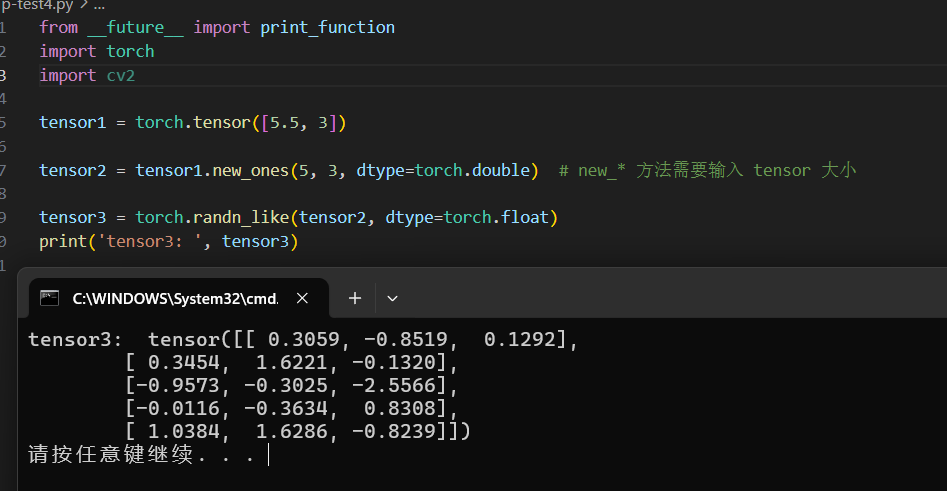
\includegraphics[width=\textwidth]{屏幕截图 2024-09-15 104036.png}
  \caption{torch.randn\_like(old\_tensor)}
\end{figure}

7.tensor1.add\_(tensor2):直接修改 tensor 变量
\begin{figure}[H]
  \centering
  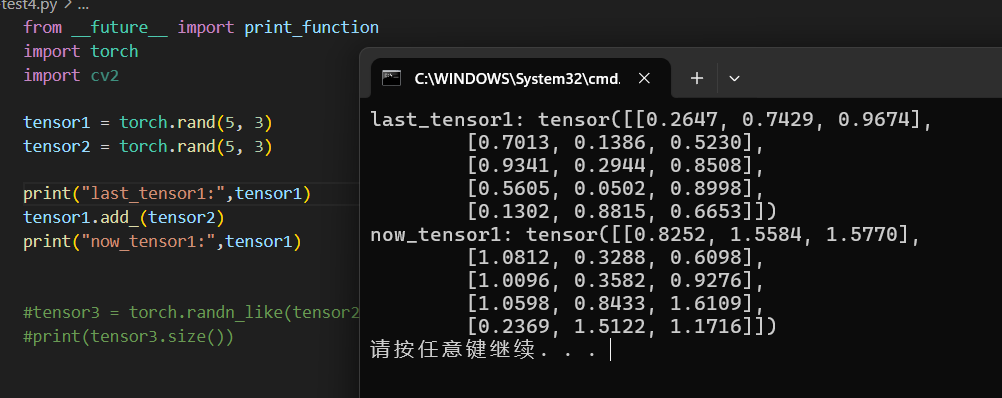
\includegraphics[width=\textwidth]{屏幕截图 2024-09-15 104649.png}
  \caption{tensor1.add\_(tensor2)}
\end{figure}

8.tensor3.size():对 tensors 的尺寸大小获取 
\begin{figure}[H]
  \centering
  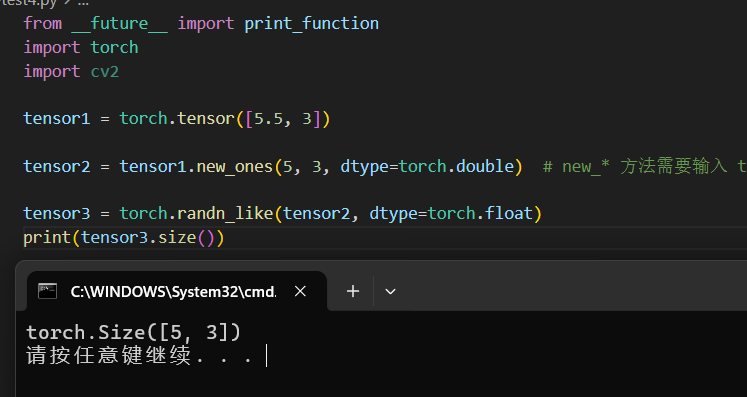
\includegraphics[width=\textwidth]{屏幕截图 2024-09-15 104310.png}
  \caption{torch.rand()}
\end{figure}

9.A.backward(torch.tensor(1.)):计算梯度
\begin{figure}[H]
  \centering
  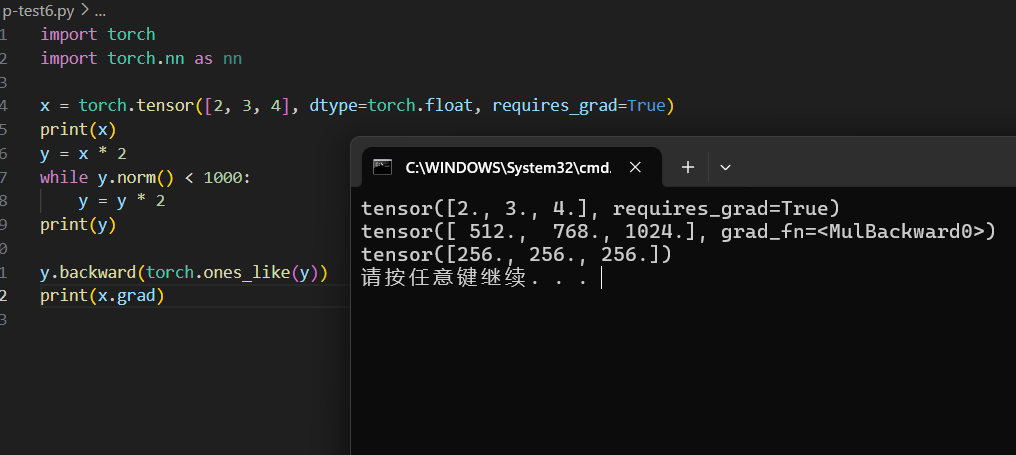
\includegraphics[width=\textwidth]{屏幕截图 2024-09-15 111829.png}
  \caption{A.backward}
\end{figure}

10.torch.range(begin,end,step):起始位置,终止位置和步长 
\begin{figure}[H]
  \centering
  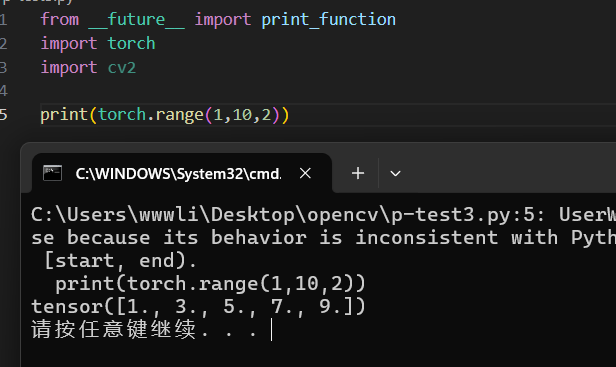
\includegraphics[width=\textwidth]{屏幕截图 2024-09-15 105412.png}
  \caption{torch.range(begin,end,step)}
\end{figure}

11.torch.mv(A,B):矩阵与向量相乘 
\begin{figure}[H]
  \centering
  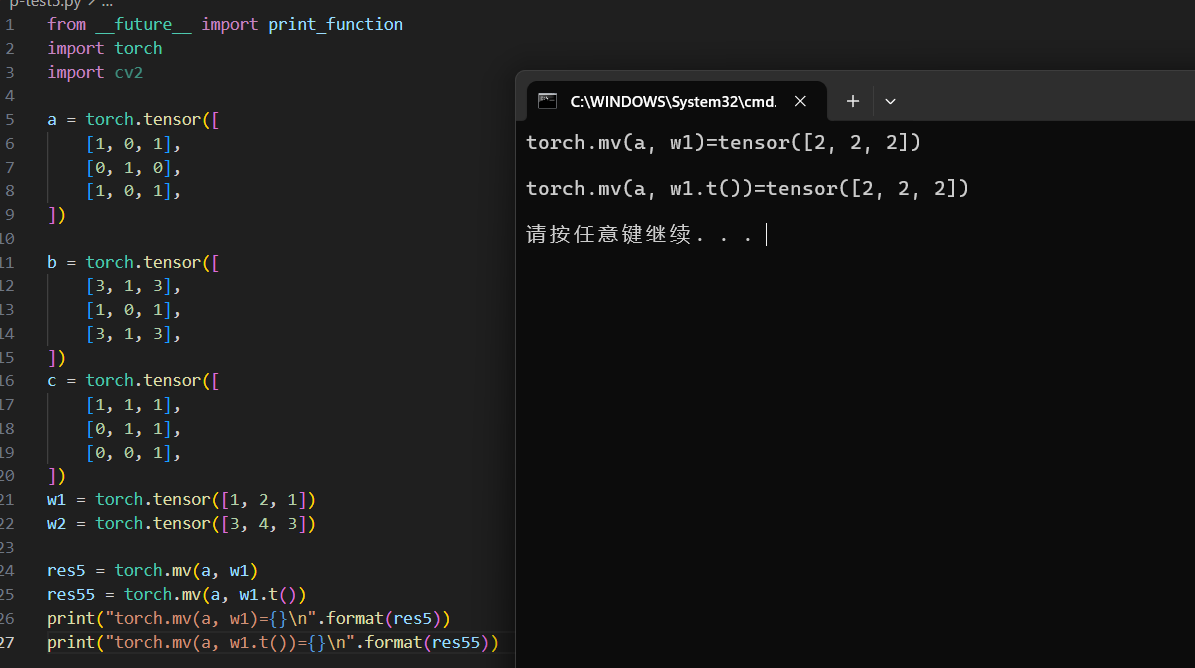
\includegraphics[width=\textwidth]{屏幕截图 2024-09-15 105721.png}
  \caption{torch.mv(A,B)}
\end{figure}

12.Tensor 转换为 Numpy 数组
\begin{figure}[H]
  \centering
  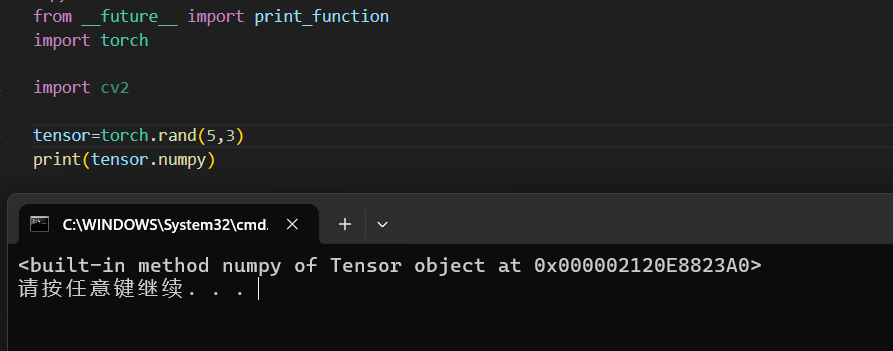
\includegraphics[width=\textwidth]{屏幕截图 2024-09-15 105945.png}
  \caption{torch.rand()}
\end{figure}




 13.torch.diag(A):取A对角线元素形成一个一维向量
\begin{figure}[H]
  \centering
  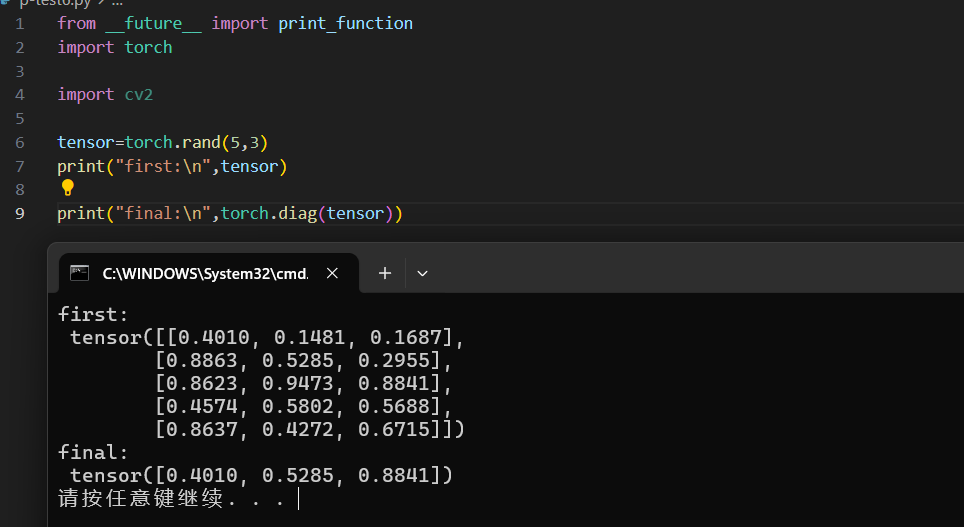
\includegraphics[width=\textwidth]{屏幕截图 2024-09-15 110200.png}
  \caption{torch.diag(A)}
\end{figure}

14.A.transpose(0,1):行列交换
\begin{figure}[H]
  \centering
  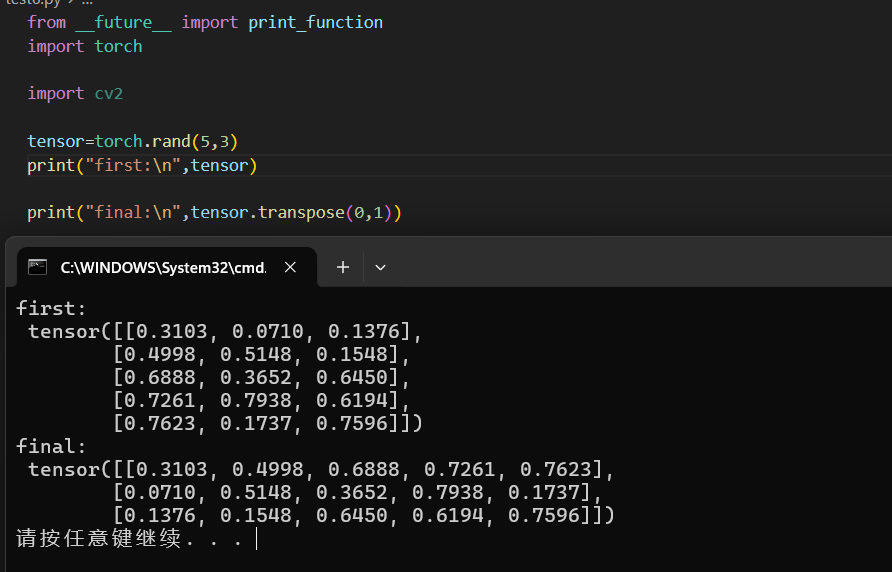
\includegraphics[width=\textwidth]{屏幕截图 2024-09-15 110337.png}
  \caption{A.transpose(0,1)}
\end{figure}

 15.torch.stack:拼接+升维
\begin{figure}[H]
  \centering
  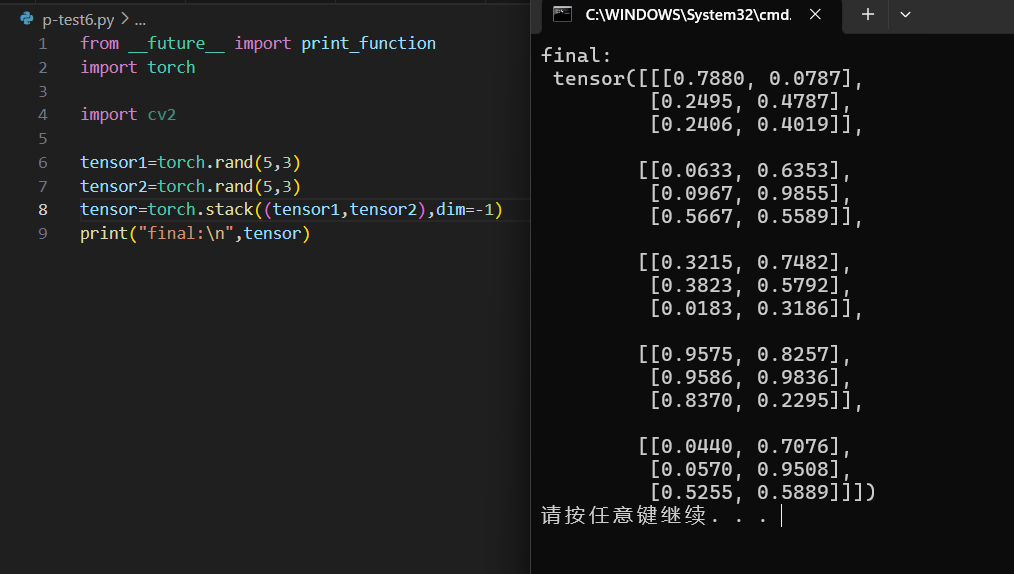
\includegraphics[width=\textwidth]{屏幕截图 2024-09-15 110619.png}
  \caption{torch.stack}
\end{figure}

16.torch.autograd.grad:求导
\begin{figure}[H]
  \centering
  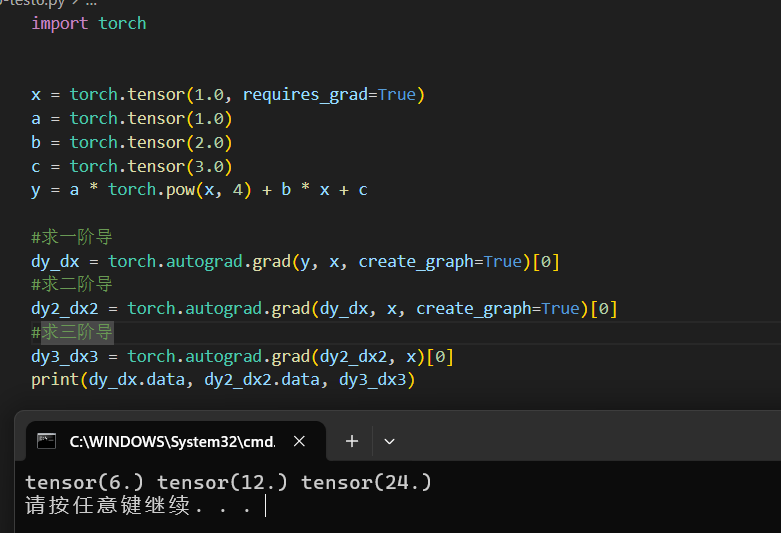
\includegraphics[width=\textwidth]{屏幕截图 2024-09-15 110908.png}
  \caption{torch.autograd.grad}
\end{figure}




\section{个人心得}

在深度学习中,性能调试对于提升模型训练效率和节省计算资源至关重要。通过合理的性能优化,能显著减少训练时间并降低硬件压力。尤其是使用 PyTorch 时,了解其 GPU 加速、混合精度训练和数据加载优化等功能,可以有效提升模型的运行速度,避免资源浪费。
\\
\indent PyTorch 提供了多种性能优化手段。首先,充分利用 GPU 并减少 CPU 和 GPU 之间的数据传输是基本操作。其次,通过梯度累加和混合精度训练能减少显存消耗,提升训练速度。此外,优化数据加载,增加并行处理的线程数量,也能明显提升效率。
\\
\indent 性能调试工具是优化的关键。PyTorch Profiler 是官方提供的性能分析工具,能深入分析每个操作的执行时间和内存占用。结合 TensorBoard 等可视化工具,可以直观地查看模型在训练中的表现,并快速定位瓶颈,从而针对性地优化。
\\
\indent 学习性能调试时,应先理解模型训练中的基本原理,逐步从小规模实验开始,然后扩展到复杂模型。同时,保持对 PyTorch 社区更新的关注,有助于学习到新的调试和优化方法,以便在实际应用中取得更好的效果。

\section{github链接}

\href{https://github.com/newbeginnerlzh/git-task01.git}{\color{red}https://github.com/newbeginnerlzh/git-task01.git}

\end{document}
